\documentclass{beamer}

\mode<presentation> 
\usetheme{Warsaw}
\usepackage{amsmath}
\usepackage{amssymb}
\usepackage{comment}

\useinnertheme{rectangles}
\useoutertheme{infolines}
% centaur logo color: 174,191,219
%\usecolortheme[RGB={134,151,179}]{structure}
% \usecolortheme[RGB={114,125,149}]{structure}
% \usecolortheme[RGB={100, 0, 0}]{structure}
\usecolortheme[RGB={66,101,144}]{structure}
\definecolor{Highlight}{rgb}{0,0,1}
\definecolor{darkgreen}{rgb}{0,.5,0}
\definecolor{darkred}{rgb}{0.5,0,0}
\definecolor{CodeColor}{rgb}{.0, .0, .4}
\newcommand{\Highlight}[1]{{\color{Highlight}#1}}
\newcommand{\Red}[1]{{\color{darkred}#1}}
\newcommand{\Green}[1]{{\color{darkgreen}#1}}
\newcommand{\Code}[1]{{\color{CodeColor} \tt \small #1}}

\beamertemplatenavigationsymbolsempty

\usebeamerfont{title}
\usebeamerfont{author}
\usebeamerfont{institute}
\usebeamerfont{date}
\setlength{\parindent}{0pt}

\newcommand{\SmallSkip}{\vspace{0.5cm}\noindent}
\newcommand{\Skip}{\vspace{1cm}\noindent}
\newcommand{\MedSkip}{\vspace{1.5cm}\noindent}
\newcommand{\BigSkip}{\vspace{2cm}\noindent}

\AtBeginSection[] {
%% Uncomment the lines inside of here to get an extra Outline page
%% in front of each section.
% \begin{frame}
%  \frametitle{Outline}
%  \tableofcontents[currentsection]
% \end{frame}
}


\title{UBDD Library Enhancements}
\subtitle{(and other random stuff)}
\author[Page \thepage]{Jared Davis and Sol Swords}
\date{November 5, 2008}
\institute{Centaur Technology}
\logo{
\includegraphics[scale=0.31]{logo}} 

\begin{document}


\begin{comment}

Abstract for this week's ACL2 talk

Hi,

At this week's ACL2 meeting, I'll talk about some improvements that Sol Swords
and I made to the UBDD library over the summer.

UBDDs are a canonical way to represent Boolean functions introduced by Warren
Hunt and Bob Boyer.  The core UBDD operations only take up a couple of pages to
define, but when memoized they produce a fairly efficient BDD package.  Today,
UBDDs are used extensively at Centaur: they are an integral part of the "G"
system (both the current version and Sol's "GL" revision); they are also a
fundamental part of the hardware description language, E, which our analysis is
based on.

A good part of the talk will have little to do with UBDDs, but instead will be
about the supporting utilities that we have come up with.  These include:

   (1) a better alternative to deftheory, 
   (2) an automatic tool for introducing "flag" functions for mutual-recursion,
   (3) a generalization clause processor which can be useful for computed hints,
       and 
   (4) an optimization called "opportunistic laziness" which may be useful in 
       improving the efficiency of your functions

All of these are lightly used in our new version of the UBDD library, and they
are all publically available via the acl2-books repository.

The remainder of the talk will be about some new approaches we have developed
for reasoning about UBDDs.  These techniques center around the isomorphism
between a Boolean function and the set of vectors which satisfy it.  That is,
we can transform the question of whether ``f = g'' into ``f(v) = g(v) for an
arbitrary v.''  This allows us to avoid dealing with the peculiar structure of
UBDDs, and instead reason about them abstractly.  

We have developed some elaborate techniques (computed hints, clause processors,
or hints, etc.) that allow us to effectively, automatically use this approach.
As a result, we have been able to eliminate many lemmas and hints from some
previously-accomplished UBDD proofs.  Also, Sol is now using our most advanced
approach in his GL work, and it is successfully proving hundreds (thousands?)
of subgoals automatically.

Jared

\end{comment}


\maketitle
\logo{}

\begin{frame}
\frametitle{Outline}
\tableofcontents
\end{frame}

\section{Introduction to UBDDs}

\begin{frame}
\frametitle{Representations of Boolean functions}

\begin{center}
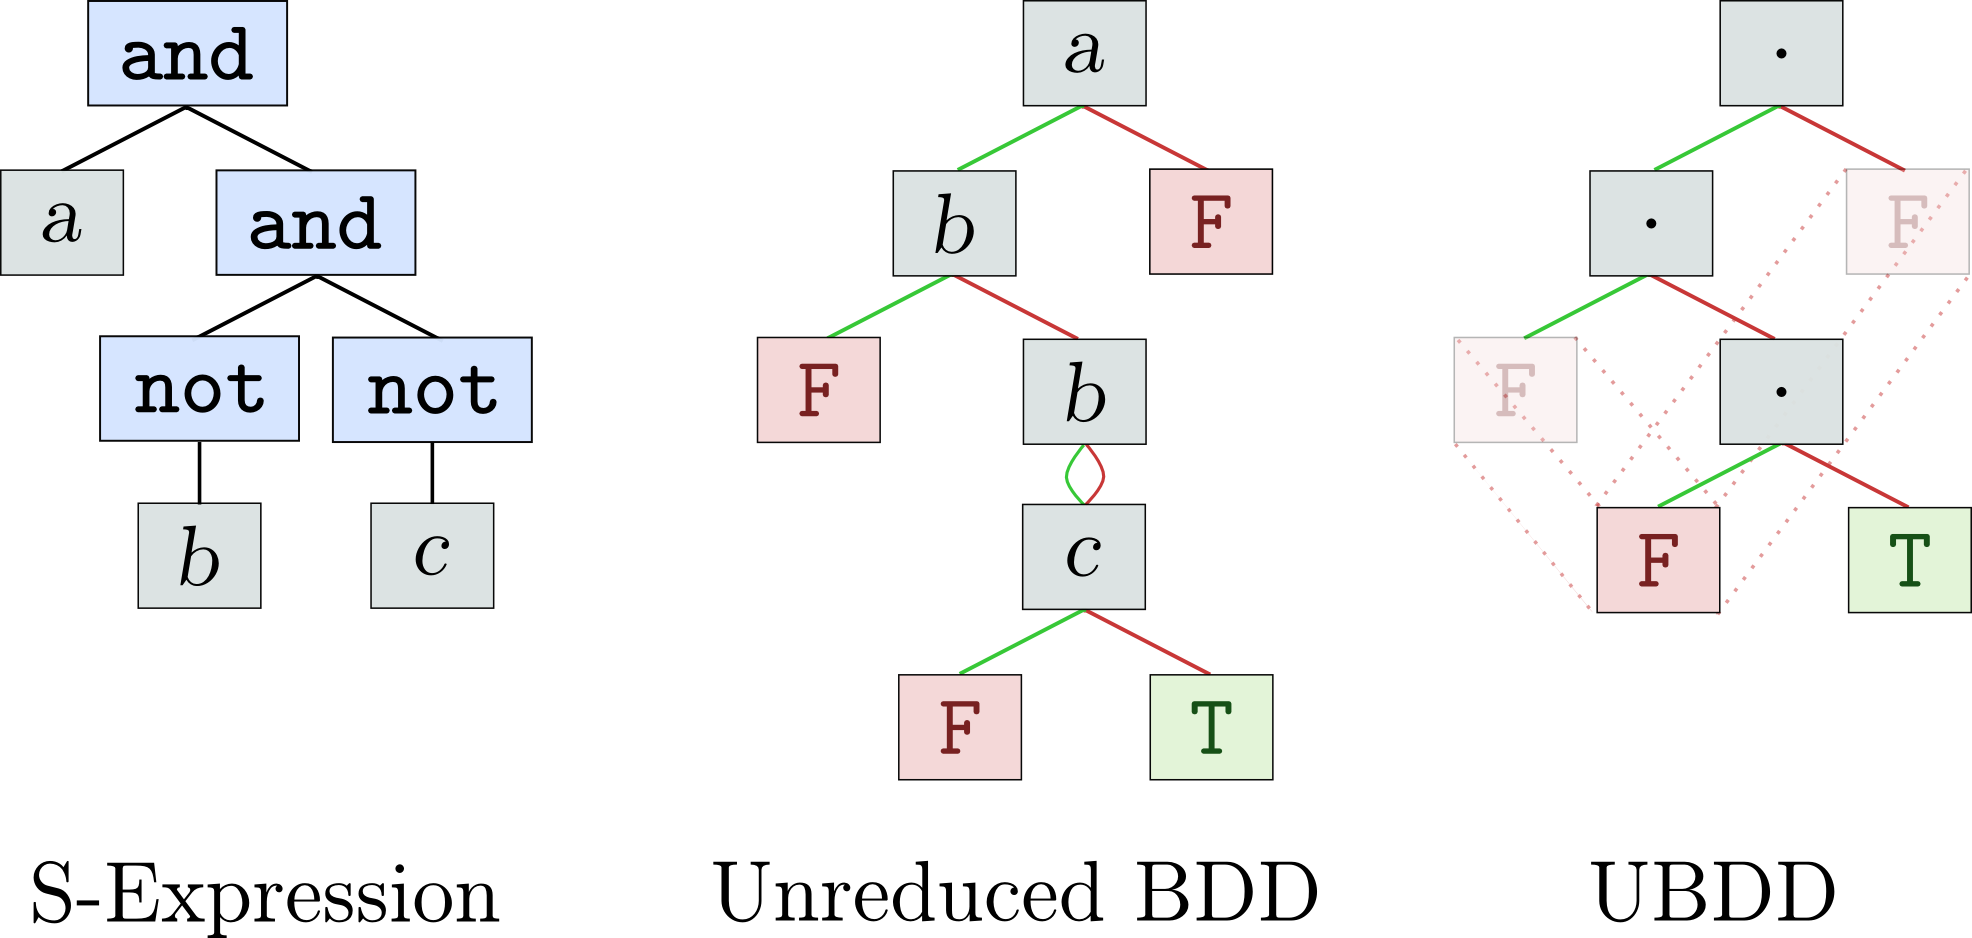
\includegraphics[width=11cm]{reps.png}
\end{center}

\end{frame}



\begin{frame}
\frametitle{Interpreting representations of Boolean functions}

In most representations, meanings are given by \Highlight{environments} mapping
variables to values

\begin{itemize}
\item \Code{(eval T env) = T}
\item \Code{(eval NIL env) = NIL}
\item \Code{(eval var env) = (lookup var env)}
\item \Code{(eval `(and ,a ,b) env) = (and (eval a env) (eval b env))}
\item \Code{(eval `(or ,a ,b) env) = (or (eval a env) (eval b env))}
\item \Code{(eval `(not ,a) env) = (not (eval a env))}
\end{itemize}

%% \SmallSkip
%% Example: if $f$ is \Code{(and a (and (not b) (not c)))}, then:
%% \begin{itemize}
%% \item \Code{(eval $f$ \{a $\leftarrow$ T, b $\leftarrow$ NIL, c $\leftarrow$ T\}) = NIL}
%% \item \Code{(eval $f$ \{a $\leftarrow$ T, b $\leftarrow$ NIL, c $\leftarrow$ NIL\}) = T}
%% \end{itemize}

\end{frame}



\begin{frame}
\frametitle{Interpreting UBDDs}

For UBDDs, meanings are given by \Highlight{list of values} telling us to go left
or right as we descend

\begin{itemize}
\item \Code{(eval-ubdd T vals) = T}
\item \Code{(eval-ubdd NIL vals) = NIL}
\item \Code{(eval-ubdd `(,a $.$ ,b) T::vals) = (eval-ubdd a vals)}
\item \Code{(eval-ubdd `(,a $.$ ,b) NIL::vals) = (eval-ubdd b vals)}
\end{itemize}

%% \SmallSkip

%% Let $f$ be \Code{(\Highlight{(NIL $.$ (NIL $.$ T))} $.$ NIL)}
%% \begin{itemize}
%% \item \Code{(eval-bdd $f$ [T, NIL, T]) = NIL}
%% \item \Code{(eval-bdd $f$ [T, NIL, NIL]) = T}
%% \end{itemize}

\end{frame}


%% \begin{frame}[fragile]
%% \frametitle{UBDDs Can Represent all Boolean Functions}

%% \begin{verbatim}
%% (defthm normp-of-q-ite
%%   (implies (and (normp a)
%%                 (normp b)
%%                 (normp c))
%%            (normp (q-ite a b c))))

%% (defthm eval-bdd-of-q-ite
%%   (equal (eval-bdd (q-ite a b c) vals)
%%          (if (eval-bdd a vals)
%%              (eval-bdd b vals)
%%            (eval-bdd c vals))))
%% \end{verbatim}
%% \end{frame}

\begin{frame}
\frametitle{Canonicity}

For UBDDs, the following statements are equivalent
\begin{itemize}
\item x = y
\item $\forall$ vals : \Code{(eval-ubdd x vals)} $=$ \Code{(eval-ubdd y vals)}
\end{itemize}

\SmallSkip
Many Boolean-function representations do not have this property
\begin{itemize}
\item \Code{(not a)} vs. \Code{(not (not (not a)))}
\end{itemize}

\SmallSkip

Efficiency characteristics
\begin{itemize}
\item Expensive to construct
\item Cheap to compare (pointer equality)
\end{itemize}

\end{frame}



\begin{frame}[fragile]
\begin{verbatim}
(defun normp (x)
  (if (atom x)
      (booleanp x)
    (and (normp (car x))
         (normp (cdr x))
         (if (atom (car x))
             (not (equal (car x) (cdr x)))
           t))))

(defun q-not (x)
  (if (atom x)
      (if x nil t)
    (hons (q-not (car x))
          (q-not (cdr x)))))
\end{verbatim}
\end{frame}


\begin{frame}[fragile]
\begin{verbatim}
(defun q-ite (x y z)
  (cond ((null x) z)
        ((atom x) y)
        (t 
         (let ((y (if (hons-equal x y) t y))
               (z (if (hons-equal x z) nil z)))
           (cond ((hons-equal y z)
                  y)
                 ((and (eq y t) (eq z nil))
                  x)
                 ((and (eq y nil) (eq z t))
                  (q-not x))
                 (t 
                  (qcons 
                   (q-ite (car x) (qcar y) (qcar z))
                   (q-ite (cdr x) (qcdr y) (qcdr z)))))))))
\end{verbatim}
\end{frame}


\begin{frame}[fragile]
\begin{verbatim}
(defun q-and (x y)
  (cond ((atom x)
         (if x 
             (if (atom y) 
                 (if y t nil) 
               y)
           nil))
        ((atom y)
         (if y x nil))
        ((hons-equal x y)
         x)
        (t
         (qcons (q-and (car x) (car y))
                (q-and (cdr x) (cdr y))))))
\end{verbatim}
\end{frame}



\section{New, generally useful stuff}

\begin{frame}
\frametitle{Outline} \tableofcontents[currentsection]
\end{frame}


\subsection{Opportunistic laziness}

\begin{frame}[fragile]
\frametitle{Opportunistic laziness}

Sometimes the result of a function call may be apparent even without evaluating
all of its arguments
\begin{itemize}
\item \Code{(* (fib x) 0)}
\item \Code{(difference nil (mergesort x))}
\item \Code{(q-and nil (q-not x))}
\end{itemize}

\SmallSkip
Matt has improved MBE to facilitate this
\begin{itemize}
\item Defthm has improved awareness of MBE
\item Restrictions on nested MBEs have been loosened
\item Induction schemes may still have some issues
\end{itemize}

\end{frame}


\begin{frame}[fragile]
\frametitle{A simple example: q-ite}

Avoid evaluating \Code{y} or \Code{z} when \Code{x} evaluates to a constant

\begin{verbatim}
(defmacro q-ite (x y z) 
  `(mbe :logic (q-ite-fn ,x ,y ,z)
        :exec (let ((_x ,x))
                (cond ((null _x) ,z)
                      ((atom _x) ,y)
                      (t
                       (q-ite-fn _x ,y ,z)))))))

(add-macro-alias q-ite q-ite-fn)
(add-untranslate-pattern (q-ite-fn ?x ?y ?z)
                         (q-ite ?x ?y ?z))
\end{verbatim}
\end{frame}



\begin{frame}
\frametitle{Identifying additional opportunities}

In \Code{(q-and x$_1$ x$_2$ $\dots$ x$_n$)}, when any \Code{x$_i$} $=$ \Code{NIL}
then the answer is \Code{NIL}

\SmallSkip

Which order should we use?
\begin{itemize}
\item \Code{(q-and nil (q-not y))}
\item \Code{(q-and (q-not x) y)}
\item \Code{(q-and (q-not x) (q-not y))}
\end{itemize}

\SmallSkip
Surely cheap
\begin{itemize}
\item quoted constants, (``don't need to be evaluated'')
\item variables, (``already evaluated'')
\end{itemize}

\SmallSkip 
So we evaluate the surely-cheap arguments first
\end{frame}

\subsection{Rulesets}

\begin{frame}[fragile] 
\frametitle{Rulesets}

\Highlight{Rulesets} are extensible deftheories
\begin{itemize}
\item \Code{(include-book "tools/rulesets" :dir :system)}
\end{itemize}

\SmallSkip
Defining and extending rulesets
\begin{itemize}
\item \Code{(def-ruleset foo '(car-cons cdr-cons))}
\item \Code{(add-to-ruleset foo '(default-car default-cdr))}
\end{itemize}

\SmallSkip
Enabling and disabling rulesets
\begin{itemize}
\item \Code{(in-theory (enable* (:ruleset foo)))}
\item \Code{(in-theory (disable* append (:ruleset foo) reverse))}
\item \Code{(in-theory (e/d* (reverse member) ((:ruleset foo))))}
\end{itemize}
\end{frame}



\begin{frame}[fragile] 
\frametitle{Ruleset fanciness}

Rulesets can contain pointers to other rulesets
\begin{itemize}
\item \Code{(def-ruleset foo '(car-cons))}
\item \Code{(def-ruleset bar '(cdr-cons (:ruleset foo)))}
\end{itemize}

\SmallSkip
These really are like pointers
\begin{itemize}
\item \Code{(add-to-ruleset foo '(append))}
\item \Code{(in-theory (disable* (:ruleset bar)))} ;; append is disabled
\end{itemize}

\SmallSkip
If you use your own package, it's easy to make \Code{FOO::enable} be an alias to
\Code{enable*}, etc.


\end{frame}

\subsection{Make-flag}

\begin{frame}[fragile] 
\frametitle{Make-flag}

\Highlight{Make-flag} generates a flag function for a mutual-recursion
\begin{itemize}
\item Non-executable; multiple-values and stobjs are fine
\item Measure inferred from existing definitions
\item Efficient proof of equivalence theorem
\item Adds a macro for proving new theorems about these functions
\end{itemize}
\end{frame}



\begin{frame}[fragile] 
\frametitle{Make-flag example}

\begin{verbatim}
(include-book "tools/flag" :dir :system)

(FLAG::make-flag flag-pseudo-termp
                 pseudo-termp
                 :flag-var flag
                 :flag-mapping ((pseudo-termp . term)
                                (pseudo-term-listp . list))
                 :hints(( {for the measure theorem} ))
                 :defthm-macro-name defthm-pseudo-termp)

(defthm-pseudo-termp type-of-pseudo-termp
  (term (booleanp (pseudo-termp x)))
  (list (booleanp (pseudo-term-listp lst)))
  :hints(("Goal" :induct (flag-pseudo-termp flag x lst))))
\end{verbatim}
\end{frame}

\subsection{Generalization clause processor}

\begin{frame}[fragile] 
\frametitle{Generalization clause processor}

\Highlight{Simple-generalize-cp} lets you specify how a clause should be
generalized

{\footnotesize \begin{verbatim}
(include-book "clause-processors/generalize" :dir :system)

(defstub foo (x) x)
(defstub bar (x) x)

(thm (equal (foo x) (bar y))
  :hints(("Goal"
          :clause-processor
          (simple-generalize-cp clause '(((bar y) . z))))))

We now apply the verified :CLAUSE-PROCESSOR function SIMPLE-GENERALIZE-
CP to produce one new subgoal.

Goal'
(EQUAL (FOO X) Z).
\end{verbatim}}
\end{frame}

\begin{frame}[fragile] 
\frametitle{Supporting hint-directed generalization}

Tools for generating fresh variables
\begin{itemize}
\item \Code{(make-n-vars n root m avoid)}
\item \Code{(term-vars x)} and \Code{(term-vars-list x)}
\end{itemize}

\SmallSkip
Examples:
\begin{verbatim}
  ACL2 !>(make-n-vars 3 'foo 0 '(x y z foo0 foo1 foo2))
  (FOO3 FOO4 FOO5)

  ACL2 !>(term-vars '(if x y z))
  (X Y Z)
\end{verbatim}

\end{frame}



\section{Reasoning about UBDDs}
\begin{frame}
\frametitle{Outline} \tableofcontents[currentsection]
\end{frame}


\subsection{Pick-a-point proofs}
\begin{frame}
\frametitle{Reasoning about UBDDs}

Why do we care?

\SmallSkip
No ACL2 reasoning is needed for equivalence checking
\begin{itemize} 
\item Build a UBDD for the circuit (execution)
\item Build a UBDD for the specification (execution)
\item Check if they are equal (execution)
\end{itemize}

\SmallSkip

But there are other, critical uses of UBDDs
\begin{itemize}
\item Parameterization --- partitions an input space into UBDDs
\item AIG conversion --- builds a UBDD from an AIG
\item G System --- represents symbolic objects as lists of UBDDs
\end{itemize}

\end{frame}




\begin{frame}[fragile]
\frametitle{The direct approach}

The ``recursion and induction'' approach does not work very well

\SmallSkip
Some problems
\begin{itemize}
\item Finding workable induction schemes
\item Case-splits in UBDD construction (\Code{q-car}, \Code{q-cdr}, \Code{q-cons})
\end{itemize}

\SmallSkip
It also ``feels wrong''
\begin{itemize}
\item Structural, low-level view of Boolean functions
\item Not applicable to other representations (AIGs, ...)
\end{itemize}

\SmallSkip
Similar to the problem of reasoning about ordered sets

\end{frame}


\begin{frame}[fragile]
\begin{verbatim}
(defthm q-and-equiv
  (implies (and (normp x)
                (normp y))
           (equal (q-and x y)
                  (q-ite x y nil))))
\end{verbatim}
ACL2 can do the proof directly (0.7s)
\begin{itemize}
\item Merges induction schemes of \Code{normp} and \Code{q-ite}
\item *1/22 inductive subgoals
\item Many subsequent case splits
\end{itemize}


\end{frame}

\begin{frame}[fragile]
\begin{verbatim}
(defun q-xor (x y)
  (cond ((atom x)
         (if x (q-not y) y))
        ((atom y)
         (if y (q-not x) x))
        ((hons-equal x y)
         nil)
        (t
         (qcons (q-xor (car x) (car y))
                (q-xor (cdr x) (cdr y))))))

(defthm q-xor-equiv
  (implies (and (normp x)
                (normp y))
           (equal (q-xor x y)
                  (q-ite x (q-not y) y))))
\end{verbatim}
\end{frame}

\begin{frame}[fragile]
\small{\begin{verbatim}
Subgoal *1/7.97.164.8'
(IMPLIES (AND (CONSP X)
              Y (CONSP Y)
              (NOT (EQUAL X (Q-NOT Y)))
              (NOT (EQUAL (Q-NOT Y) Y))
              (EQUAL (Q-ITE (CAR X) (CAR (Q-NOT Y)) NIL)
                     T)
              (NOT (EQUAL (Q-ITE (CDR X) (CDR (Q-NOT Y)) (CDR Y))
                          T))
              (NOT (CAR Y))
              (CDR Y)
              (CONSP (CDR Y))
              (EQUAL (Q-XOR (CDR X) (CDR Y))
                     (Q-ITE (CDR X) (Q-NOT (CDR Y)) (CDR Y)))
              (NORMP (CAR X))
              (NORMP (CDR X))
              (CONSP (CAR X))
              (NORMP (CDR Y))
              (NOT (EQUAL (Q-NOT Y) T)))
         (NOT (Q-NOT Y)))
\end{verbatim}}
\end{frame}


\begin{frame}
\frametitle{Pick-a-point proofs}

{\bf Prove}: $(A \cup B) \cap C = (A \cap C) \cup (B \cap C)$

\SmallSkip
{\bf Proof}: Let $x$ be an arbitrary element.  We will show $x$ is in $(A \cup B)
\cap C$ exactly when it is in $(A \cap C) \cup (B \cap C)$.

\begin{eqnarray*}
x \in \Red{(A \cup B)} \cap \Green{C}
  &\leftrightarrow& \Red{(x \in A \cup B)} \wedge \Green{x \in C} \\
  &\leftrightarrow& \Red{(x \in A \vee x \in B)} \wedge \Green{x \in C}
\end{eqnarray*}
\begin{eqnarray*}
x \in \Red{(A \cap C)} \cup \Green{(B \cap C)}
  &\leftrightarrow& \Red{x \in A \cap C} \vee \Green{x \in B \cap C} \\
  &\leftrightarrow& \Red{(x \in A \wedge x \in C)} \vee \Green{(x \in B \wedge x \in C)} \\
  &\leftrightarrow& (\Red{x \in A} \vee \Green{x \in B}) \wedge x \in C
\end{eqnarray*}
Q.E.D.
\end{frame}


\begin{frame}
\frametitle{Pick-a-point proofs of UBDDs}

{\bf Sets} \[x = y \leftrightarrow \forall a : \mathit{has}(x, a) = \mathit{has}(y, a)\]

\SmallSkip
{\bf UBDDs} \[x = y \leftrightarrow \forall a : \mathit{eval\textrm{-}bdd}(x,
a) = \mathit{eval\textrm{-}bdd}(y, a)\]

\SmallSkip
Some familiar set-theory operations
\begin{itemize}
\item \Code{NIL}, the empty set
\item \Code{T}, the universal set
\item \Code{Q-NOT}, set complement
\item \Code{Q-AND}, set intersection
\item \Code{Q-OR}, set union
\end{itemize}
\end{frame}



\begin{frame}[fragile]
\frametitle{Osets-style automation}

Suppose \Code{(bdd-lhs)}, \Code{(bdd-rhs)}, and \Code{(bdd-hyp)} satisfy
\begin{verbatim}
  (implies (and (bdd-hyp)
                (normp (bdd-lhs))
                (normp (bdd-rhs)))
           (equal (eval-bdd (bdd-lhs) vals) 
                  (eval-bdd (bdd-rhs) vals)))
\end{verbatim}

\SmallSkip
Then, we can prove
\begin{verbatim}
  (implies (and (bdd-hyp) 
                (normp (bdd-lhs))
                (normp (bdd-rhs)))
           (equal (bdd-lhs) (bdd-rhs)))
\end{verbatim}

\SmallSkip
A default hint functionally instantiates this theorem when our goal is to show
two \Code{normp}'s are equal (and other approaches have failed)
\end{frame}


\begin{frame}[fragile]
\frametitle{Preparing for pick-a-point proofs}

For ordered sets
\begin{itemize}
\item \Code{(setp (union x y))}
\item \Code{(in a (union x y))} $=$ \Code{(in a x)} $\vee$ \Code{(in a y)}
\end{itemize}

\SmallSkip

For UBDDs
\begin{itemize}
\item \Code{(normp x)}, \Code{(normp y)} $\rightarrow$ \Code{(normp (q-or x y))}
\item \Code{(eval-bdd (q-or x y) a)} $=$ \Code{(eval-bdd x a)} $\vee$ \Code{(eval-bdd y a)}
\end{itemize}

\SmallSkip
These proofs are done in the ``recursion and induction'' style

They tend to be easy

\end{frame}



\begin{frame}[fragile]

{\footnotesize \begin{verbatim}
(add-bdd-fn q-and)

(defthm q-and-equiv
  (implies (and (normp x)
                (normp y))
           (equal (q-and x y)
                  (q-ite x y nil))))

We now appeal to EQUAL-BY-EVAL-BDDS in an attempt to show that (Q-AND X Y)
and (Q-ITE X Y NIL) are equal because all of their evaluations under
EVAL-BDD are the same.  (You can disable EQUAL-BY-EVAL-BDDS to avoid
this.  See :doc EQUAL-BY-EVAL-BDDS for more details.)

We augment the goal with the hypothesis provided by the :USE hint.
The hypothesis can be derived from EQUAL-BY-EVAL-BDDS via functional
instantiation, provided we can establish the constraint generated;
the constraint can be simplified using case analysis.  We are left
with the following two subgoals.
\end{verbatim}}

\end{frame}




\begin{frame}[fragile]

{\footnotesize \begin{verbatim}

Subgoal 2
(IMPLIES (AND (IMPLIES (AND (AND (NORMP X) (NORMP Y))
                            (NORMP (Q-AND X Y))
                            (NORMP (Q-ITE X Y NIL)))
                       (EQUAL (EQUAL (Q-AND X Y) (Q-ITE X Y NIL))
                              T))
              (NORMP X)
              (NORMP Y))
         (EQUAL (Q-AND X Y) (Q-ITE X Y NIL))).

But simplification reduces this to T, using the :executable-counterparts
of EQUAL and NORMP, primitive type reasoning, the :rewrite rules NORMP-
OF-Q-AND and NORMP-OF-Q-ITE and the :type-prescription rule NORMP.

\end{verbatim}}
\end{frame}


\begin{frame}[fragile]

{\footnotesize \begin{verbatim}
Subgoal 1
(IMPLIES (AND (NORMP X)
              (NORMP Y)
              (EQUAL (LEN ARBITRARY-VALUES)
                     (MAX (MAX-DEPTH (Q-AND X Y))
                          (MAX-DEPTH (Q-ITE X Y NIL))))
              (BOOLEAN-LISTP ARBITRARY-VALUES)
              (NORMP (Q-AND X Y))
              (NORMP (Q-ITE X Y NIL)))
         (EQUAL (EVAL-BDD (Q-AND X Y) ARBITRARY-VALUES)
                (EVAL-BDD (Q-ITE X Y NIL) ARBITRARY-VALUES))).

But simplification reduces this to T, using the :definition MAX, the
:executable-counterpart of NORMP, primitive type reasoning, the :rewrite
rules EVAL-BDD-OF-NON-CONSP-CHEAP, EVAL-BDD-OF-Q-AND, EVAL-BDD-OF-Q-
ITE, NORMP-OF-Q-AND and NORMP-OF-Q-ITE and the :type-prescription rule
NORMP.

Q.E.D.
\end{verbatim}}
\end{frame}


\subsection{A subset-oriented approach}

\begin{frame}[fragile]
\frametitle{A subset-oriented approach}

Our simple pick-a-point approach sometimes led to goals whose hypotheses were
difficult to use effectively

\begin{verbatim}
  (IMPLIES (AND (NORMP C)
                (NORMP HYP)
                (Q-ITE C HYP NIL)
                (NOT (EQUAL (Q-ITE C HYP NIL) HYP))
                HYP
                (NOT (EQUAL C T))
                (NOT (Q-ITE C NIL HYP))
                (NOT (EVAL-BDD C ARBITRARY-VALUES)))
           (NOT (EVAL-BDD HYP ARBITRARY-VALUES))))
\end{verbatim}
\end{frame}


\begin{frame}[fragile]
\frametitle{A graphical view}

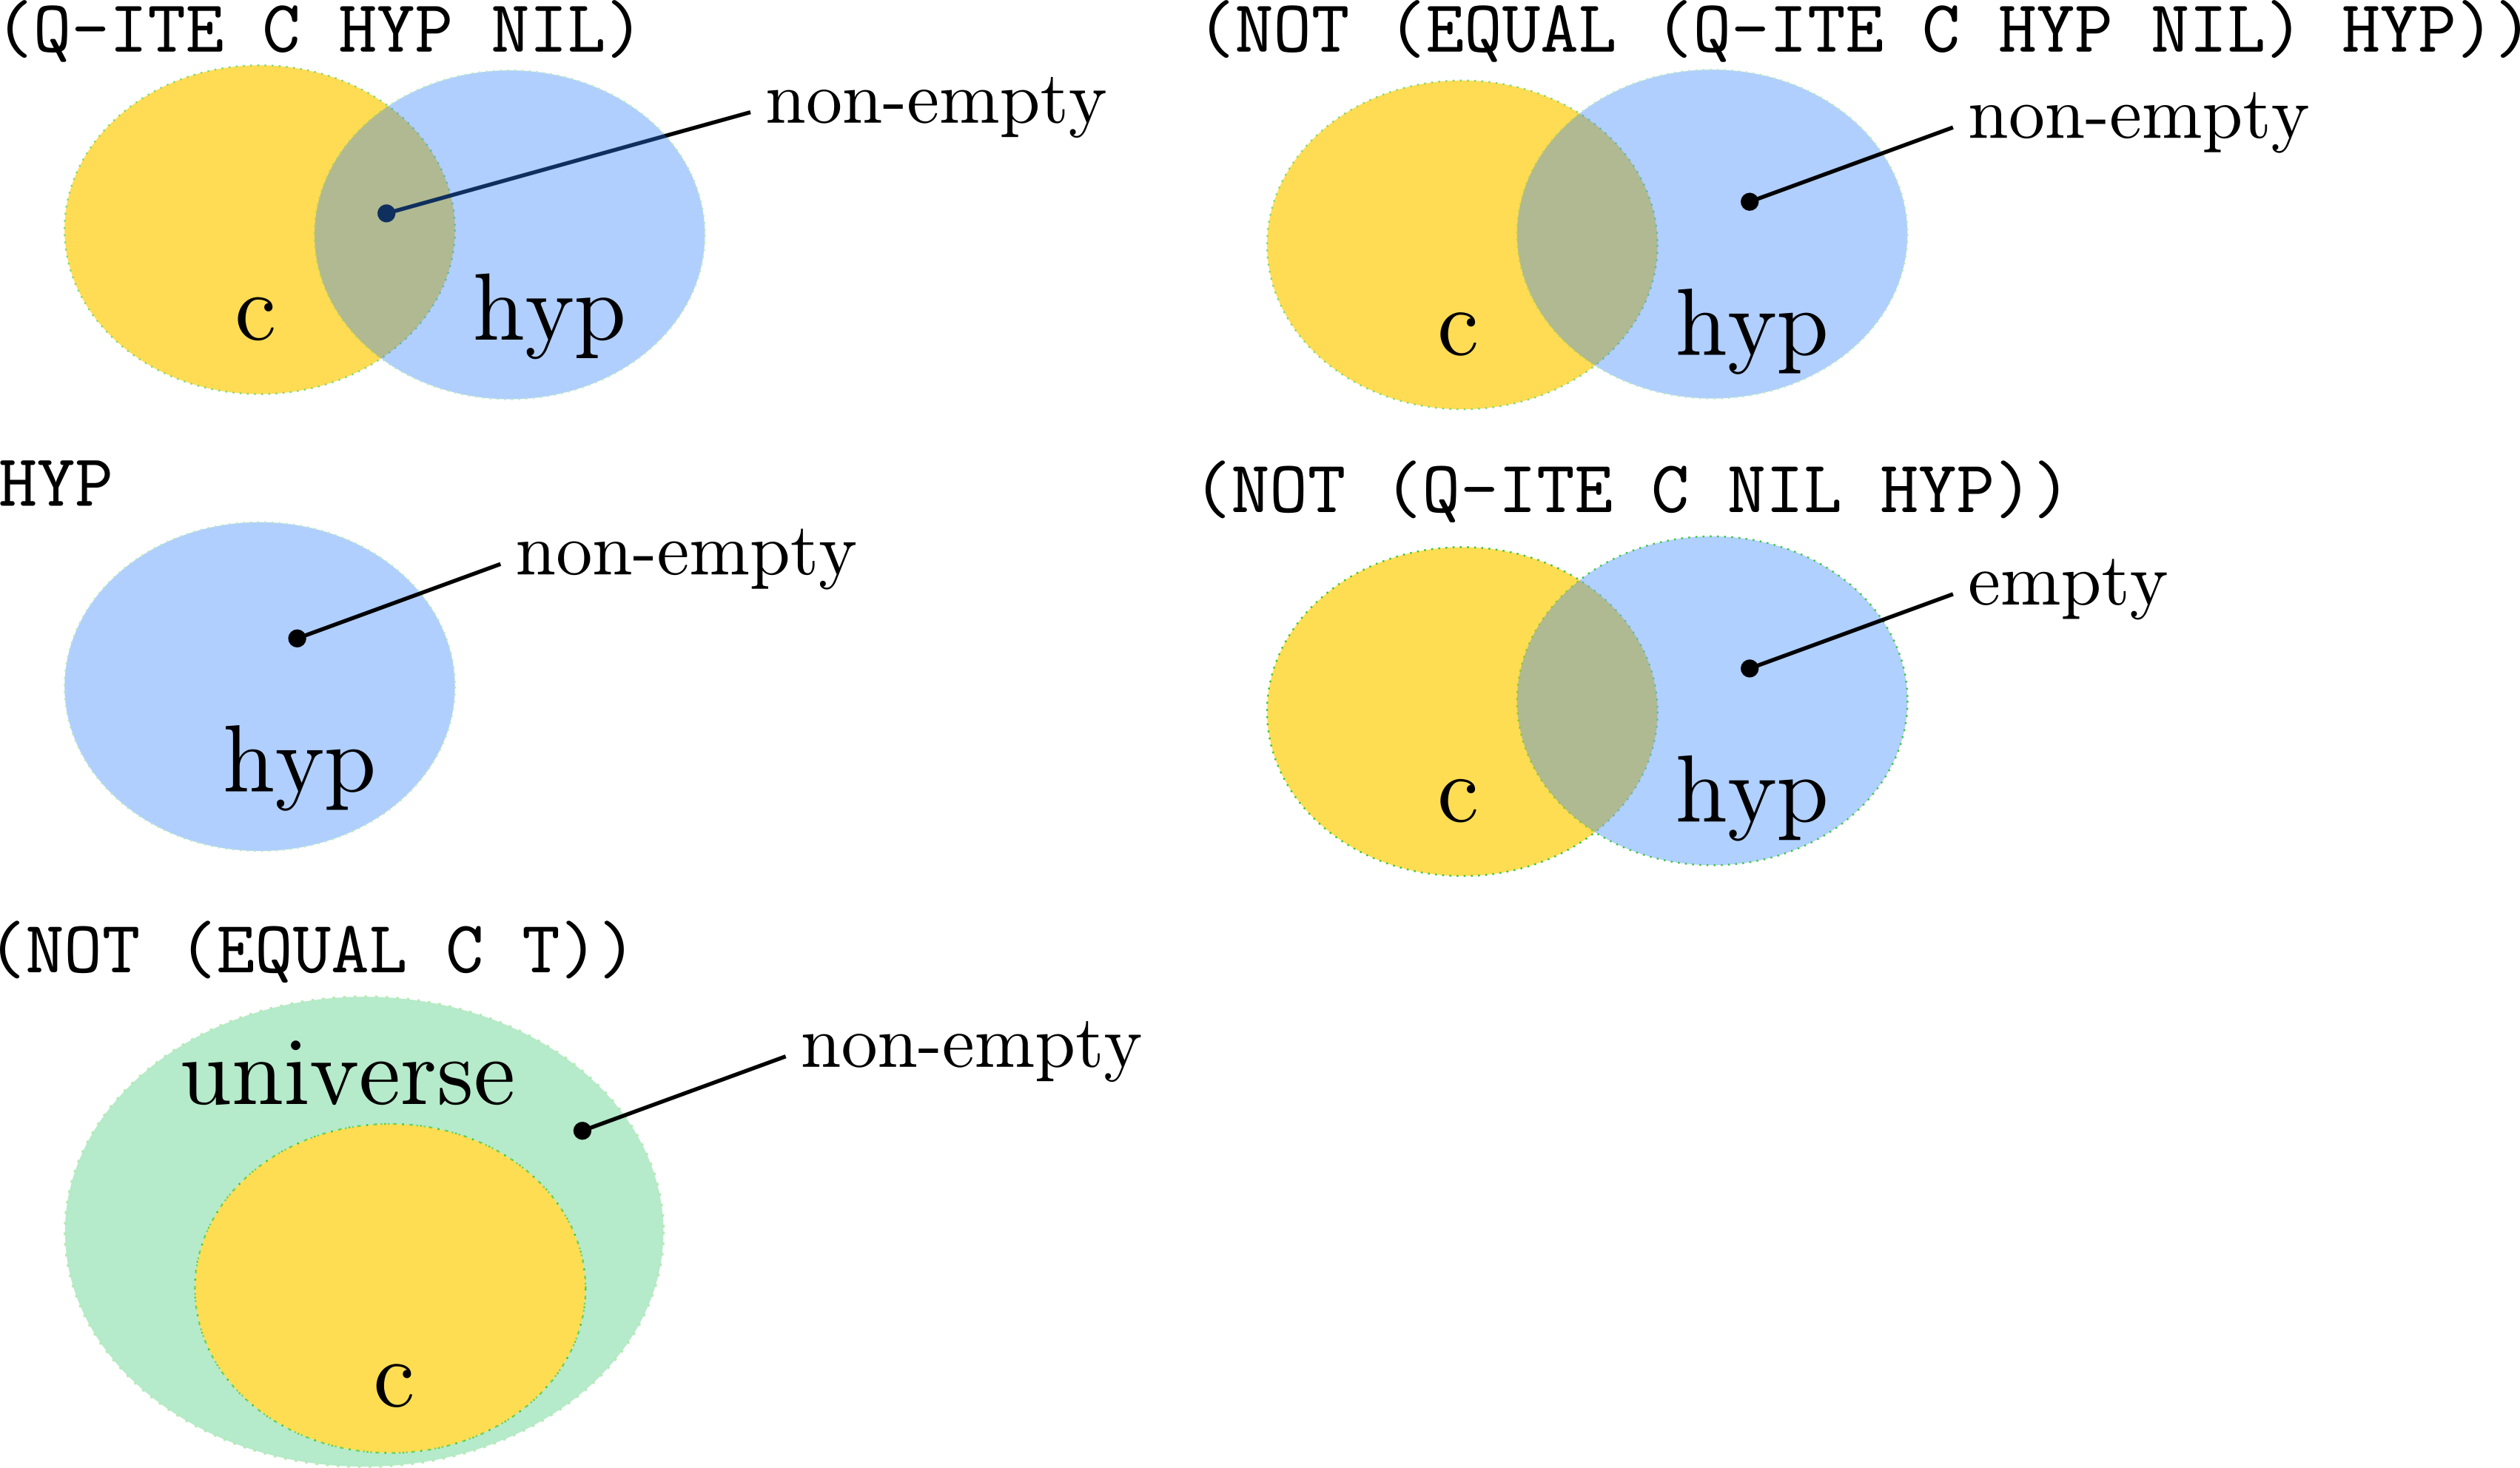
\includegraphics[width=12cm]{venn-diagrams}

\end{frame}



\begin{frame}[fragile]
\frametitle{Subset mode}

\Code{(qs-subset x y)}: $\forall$ \Code{vals} $:$ \Code{(eval-bdd x vals)} $\rightarrow$ \Code{(eval-bdd y vals)}

\begin{itemize}
\item Good properties: reflexive, transitive, membership-preserving
\item Similar pick-a-point approach for proving qs-subset
\end{itemize}

\SmallSkip
\Code{(QS-SUBSET-MODE T)} -- an alternate normal form
\begin{itemize}
\item \Code{(equal x y)} $\Rightarrow$ \Code{(qs-subset x y)} $\wedge$ \Code{(qs-subset y x)}
\item \Code{(not x)} $\Rightarrow$ \Code{(qs-subset x nil)}
\item \Code{x} $\Rightarrow$ \Code{(not (qs-subset x nil))} \\
\quad
\item \Code{(qs-subset (q-and x y) x)}
\item \Code{(qs-subset (q-and x y) y)}
\item \Code{(qs-subset x (q-or x y))}
\item \Code{(qs-subset y (q-or x y))}
\end{itemize}
\end{frame}



\begin{frame}[fragile]
\frametitle{Rewrite rules for subset mode (without {\tt normp} hyps)}
\begin{verbatim}
(equal (qs-subset w (q-ite x y z))
       (and (qs-subset (q-ite w x nil) y)
            (qs-subset (q-ite x nil w) z)))

(implies (and (syntaxp (not (equal y ''nil)))
              (syntaxp (not (equal z ''nil))))
         (equal (qs-subset (q-ite x y z) w)
                (and (qs-subset (q-ite x y nil) w)
                     (qs-subset (q-ite x nil z) w))))

(equal (qs-subset (q-ite x nil y) x)
       (qs-subset y x))

(equal (qs-subset (q-ite x nil y) nil)
       (qs-subset y x))
\end{verbatim}
\end{frame}


\begin{frame}[fragile]
\frametitle{Subset mode in action}

\Code{(not (equal (q-ite c hyp nil) hyp))} $\rightarrow$ \Code{(not (qs-subset hyp c))}
{\footnotesize \begin{verbatim}
  (not (equal (q-ite c hyp nil) hyp))
  ==> (not (and 1. (qs-subset (q-ite c hyp nil) hyp)
                   ==> t
                2. (qs-subset hyp (q-ite c hyp nil))))
                   ==> (and 2a. (qs-subset (q-ite hyp c nil) hyp)
                                ==> t
                            2b. (qs-subset (q-ite c nil hyp) nil)))
                                ==> (qs-subset hyp c)
  ==> (not (qs-subset hyp c))
\end{verbatim}}


\SmallSkip
\Code{(not (q-ite c nil hyp))} $\rightarrow$ \Code{(qs-subset hyp c)}
{\footnotesize \begin{verbatim}
  (not (q-ite c nil hyp))
  ==> (qs-subset (q-ite c nil hyp) nil)
  ==> (qs-subset hyp c)
\end{verbatim}}

\end{frame}




\subsection{A witness-oriented approach}


\begin{frame}[fragile]
\frametitle{A witness-oriented approach}

Subset-mode often works in practice, but does not seem ideal
\begin{itemize}
\item Strange normal form that affects all booleans
\item Strange iff-rewrites needed for all UBDD-making functions
\item Free variables in transitivity and the preservation of membership
\item Rules about \Code{q-ite} seem somehow fragile
\end{itemize}

\SmallSkip
\Highlight{Witness-mode} is a more advanced alternative
\begin{itemize}
\item Intuitively, ``Pick all of the probably-relevant points''
\item Casts everything in terms of \Code{eval-bdd}
\item Works with existing normal forms
\end{itemize}
\end{frame}




\begin{frame}[fragile]
\frametitle{The witness approach, graphically}

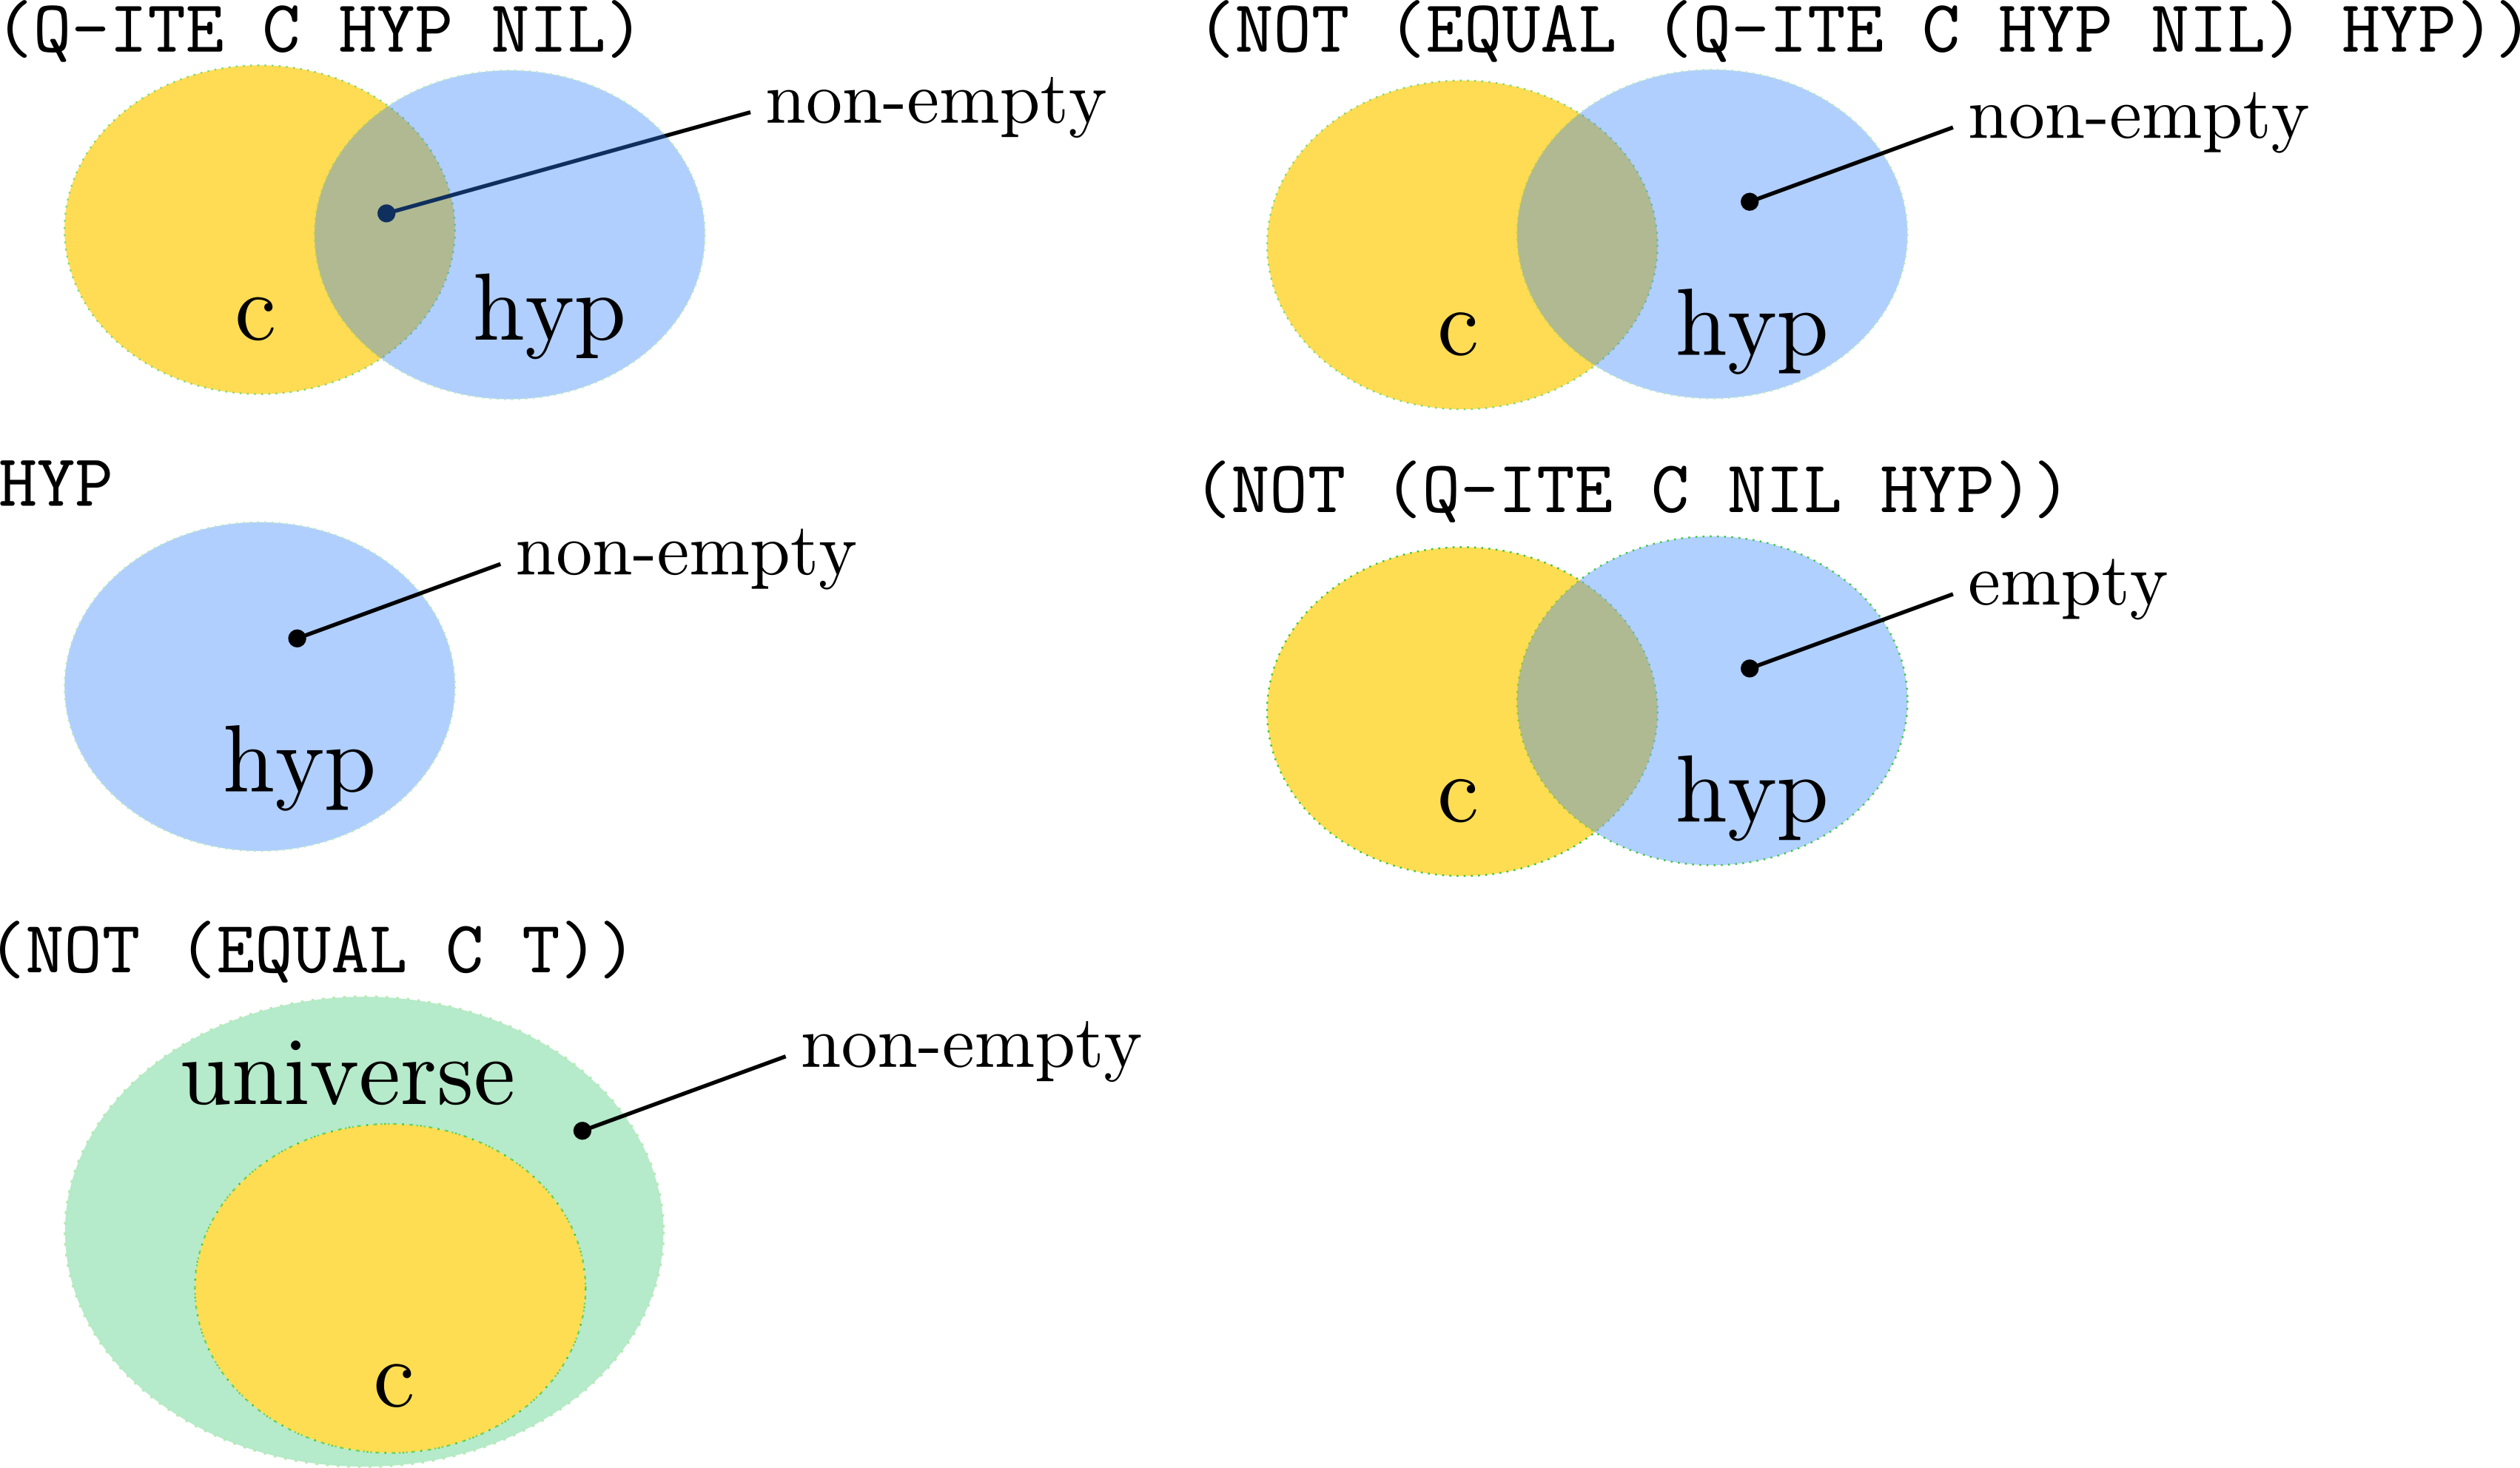
\includegraphics[width=12cm]{venn-diagrams}

\end{frame}


\begin{frame}[fragile]
\frametitle{The basic transformation}

Hypothesis: \Code{x} $\neq$ \Code{y}  (or \Code{x})
\begin{itemize}
\item Means $\exists$ \Code{v} : \Code{(eval-bdd x v)} $\neq$ \Code{(eval-bdd y v)}
\item Introduce a new variable, \Code{v}
\item Replace the hyp with \Code{(eval-bdd x v)} $\neq$ \Code{(eval-bdd y v)} 
\end{itemize}

\SmallSkip

Hypothesis: \Code{x} $=$ \Code{y}   (or \Code{(not x)})
\begin{itemize}
\item Means $\forall$ \Code{v} : \Code{(eval-bdd x v)} $=$ \Code{(eval-bdd y v)} 
\item Collect all \Code{v} occurring in the clause
\item Replace the hyp with \Code{(eval-bdd x v)} $=$ \Code{(eval-bdd y v)} 
\end{itemize}

\end{frame}


\begin{frame}[fragile]
\frametitle{Transformation example}

\begin{verbatim}
  (IMPLIES (AND ;; (NORMP C)
                ;; (NORMP HYP)
                (Q-ITE C HYP NIL)
                (NOT (EQUAL (Q-ITE C HYP NIL) HYP))
                HYP
                (NOT (EQUAL C T))
                (NOT (Q-ITE C NIL HYP))
                (NOT (EVAL-BDD C ARBITRARY-VALUES)))
           (NOT (EVAL-BDD HYP ARBITRARY-VALUES))))
\end{verbatim}

\end{frame}


\begin{frame}[fragile]

\begin{verbatim}
  (IMPLIES (AND (NOT (EQUAL (EVAL-BDD (Q-ITE C HYP NIL) V1)
                            (EVAL-BDD NIL V1)))
                (NOT (EQUAL (EVAL-BDD (Q-ITE C HYP NIL) V2)
                            (EVAL-BDD HYP V2)))
                (NOT (EQUAL (EVAL-BDD HYP V3)
                            (EVAL-BDD NIL V3)))
                (NOT (EQUAL (EVAL-BDD C V4)
                            (EVAL-BDD T V4)))
                (NOT (Q-ITE C NIL HYP))
                (NOT (EVAL-BDD C ARBITRARY-VALUES)))
           (NOT (EVAL-BDD HYP ARBITRARY-VALUES))))
\end{verbatim}

Values: \Code{V1}, \Code{V2}, \Code{V3}, \Code{V4}, \Code{ARBITRARY-VALUES}

\end{frame}


\begin{frame}[fragile]

{\footnotesize \begin{verbatim}
  (IMPLIES (AND (NOT (EQUAL (EVAL-BDD (Q-ITE C HYP NIL) V1)
                            (EVAL-BDD NIL V1)))
                (NOT (EQUAL (EVAL-BDD (Q-ITE C HYP NIL) V2)
                            (EVAL-BDD HYP V2)))
                (NOT (EQUAL (EVAL-BDD HYP V3)
                            (EVAL-BDD NIL V3)))
                (NOT (EQUAL (EVAL-BDD C V4)
                            (EVAL-BDD T V4)))

                (EQUAL (EVAL-BDD (Q-ITE C NIL HYP) V1)
                       (EVAL-BDD NIL V1))
                (EQUAL (EVAL-BDD (Q-ITE C NIL HYP) V2)
                       (EVAL-BDD NIL V2))
                (EQUAL (EVAL-BDD (Q-ITE C NIL HYP) V3)
                       (EVAL-BDD NIL V3))
                (EQUAL (EVAL-BDD (Q-ITE C NIL HYP) V4)
                       (EVAL-BDD NIL V4))
                (EQUAL (EVAL-BDD (Q-ITE C NIL HYP) ARBITRARY-VALUES)
                       (EVAL-BDD NIL ARBITRARY-VALUES))

                (NOT (EVAL-BDD C ARBITRARY-VALUES)))
           (NOT (EVAL-BDD HYP ARBITRARY-VALUES))))
\end{verbatim}}

\end{frame}


\begin{frame}[fragile]

{\small \begin{verbatim}
  (IMPLIES (AND (EVAL-BDD (Q-ITE C HYP NIL) V1)
                (NOT (EQUAL (EVAL-BDD (Q-ITE C HYP NIL) V2)
                            (EVAL-BDD HYP V2)))
                (EVAL-BDD HYP V3)
                (NOT (EVAL-BDD C V4))

                (NOT (EVAL-BDD (Q-ITE C NIL HYP) V1))
                (NOT (EVAL-BDD (Q-ITE C NIL HYP) V2))
                (NOT (EVAL-BDD (Q-ITE C NIL HYP) V3))
                (NOT (EVAL-BDD (Q-ITE C NIL HYP) V4))
                (NOT (EVAL-BDD (Q-ITE C NIL HYP) ARBITRARY-VALUES))

                (NOT (EVAL-BDD C ARBITRARY-VALUES)))
           (NOT (EVAL-BDD HYP ARBITRARY-VALUES))))
\end{verbatim}}

Follows from cases introduced by \Code{eval-bdd-of-q-ite}

\end{frame}


\begin{frame}[fragile]
\frametitle{The {\tt eval-bdd-cp} clause processor (1/2)}

\Code{(diff x y)}
\begin{itemize}
\item When \Code{x} $\neq$ \Code{y},
       \Code{(eval-bdd x (diff x y))} $\neq$ \Code{(eval-bdd y (diff x y))}
\end{itemize}

\SmallSkip
{\bf 1a.}.  Gather hyps of the form \Code{x} $\neq$ \Code{y}, where
\Code{x}, \Code{y} are (likely) UBDDs
\begin{itemize}
\item A hyp which is just \Code{x} also counts: \Code{x} $\neq$ \Code{NIL}
\end{itemize}

\SmallSkip
{\bf 1b.}.  For each \Code{x} $\neq$ \Code{y} found, replace the hyp with
\begin{center}
\Code{(implies (and (normp x) (normp y))) \qquad \qquad \qquad \qquad \qquad \qquad \quad \;} \\
\qquad \Code{(eval-bdd x (diff x y))} $\neq$ \Code{(eval-bdd y (diff x y))}
\end{center}

This is sound
\begin{itemize}
\item In the \Code{normp} case, the clauses are equivalent
\item Otherwise, the new clause implies the original
\end{itemize}

\end{frame}


\begin{frame}[fragile]
\frametitle{The {\tt eval-bdd-cp} clause processor (2/2)}

{\bf 2.} As a convenience, generalize away all \Code{(diff x y)} terms just
introduced with fresh variables. (trivially sound)

\SmallSkip
{\bf 3.} Gather up all \Code{v} which are used, anywhere, as arguments to
\Code{eval-bdd}, i.e., \Code{(eval-bdd x v)}.

\SmallSkip
{\bf 4a.} Gather hyps of the form \Code{x} $=$ \Code{y} found, where \Code{x},
\Code{y} are (likely) UBDDs
\begin{itemize}
\item A hyp which is \Code{(not x)} also counts: \Code{x} $=$ \Code{NIL}
\end{itemize}

\SmallSkip
{\bf 4b.} Replace these hyps with \Code{(eval-bdd x v)} $=$ \Code{(eval-bdd y v)}, 
for all \Code{v} found in step 3. (trivially sound)

\end{frame}



\begin{frame}[fragile]
\frametitle{Automating {\tt eval-bdd-cp}}

We use a default hint

\begin{itemize}
\item The clause must be \Code{stable-under-simplificationp}
\item The definition of \Code{eval-bdd-cp-hint} must be enabled
\item The transformation must modify the clause
\end{itemize}

\SmallSkip
The hint we give
\begin{verbatim}
(:or (:clause-processor ...)
     (:no-op t))
\end{verbatim}

\end{frame}



\section{Future directions}

\begin{frame}
\frametitle{Future directions}

Maybe: A non-UBDD convention, UBDD-fixing, and guards

\SmallSkip

Names and packages

\SmallSkip

Similar libraries for AIGs, other representations

\end{frame}


\end{document}
